\section{Results}
\label{sec:results}
The gate fails. Of its two binding conditions the first holds and the second does not, so the search was not run and no new fit was spent. Table~\ref{tab:gate} collects the scores and the damages they are checked against.

\begin{table}[htbp]
\centering
\small
\setlength{\tabcolsep}{6pt}
\renewcommand{\arraystretch}{1.08}
\begin{tabular}{@{}lrrl@{}}
\toprule
Class order & $S$ & Damage (pp) & Source of the damage \\
\midrule
Hard-tail & 895 & 1.59 \; (1.22 to 1.95) & 30 fits, pooled \\
Random, mean over 30 orders & 2,583 & 2.91 \; (2.48 to 3.34) & 30 fits, pooled \\
Random, range over 30 orders & 1,976 to 3,043 & 1.53 to 4.69 & one fit each \\
Easy-tail & 3,239 & 2.41 \; (1.95 to 2.85) & 30 fits, pooled \\
\bottomrule
\end{tabular}
\caption{The score orders the two sorted assignments correctly but places the easy-tail order above every random order, where the observed damage places it below the random average. Scores are values of Equation~\eqref{eq:score} at $\rho=100$; damages are losses of test patient-macro balanced accuracy against the balanced arm, in points, with 95 percent bootstrap intervals where the estimate pools 30 fits. The random-order damages are those of the prevalence curve, one class order per split-draw fit \citep{queisler2026prevalenceTcga}; the sorted-order damages are those of the tail-assignment study \citep{queisler2026tailTcga}.}
\label{tab:gate}
\end{table}

\noindent \textbf{G1 passes.} The easy-tail order scores 3,239 and the hard-tail order 895, so the score separates the two sorted assignments in the direction their damages take, 2.41 against 1.59 points. The margin is wide: the hard-tail order scores below every one of the 30 random orders, whose scores start at 1,976.

\noindent \textbf{G2 fails.} The mean score over the 30 random orders is 2,583, below the easy-tail order's 3,239, where the gate requires it to lie above. The failure is not marginal. No random order scores as high as the easy-tail order, the largest reaching 3,043, so the score ranks the easy-tail assignment as more damaging than every random assignment observed. The measured damages run the other way: the easy-tail order costs 2.41 points against 2.91 points for the random orders on average, and only 5 of the 30 individual random orders cost less than it does. The score's most extreme case, among the orders whose damage is known, is one of the milder cases in fact.

\noindent \textbf{G3 is positive.} Across the 30 random orders the score and the observed damage correlate at a Spearman coefficient of 0.38 ($p=0.04$, $n=30$). The score therefore does carry signal about damage within that family of orders, which makes the failure of G2 sharper rather than softer: the quantity tracks damage among random assignments and inverts it for the one assignment family that is known to lie outside them.

\begin{figure}[htbp]
\centering
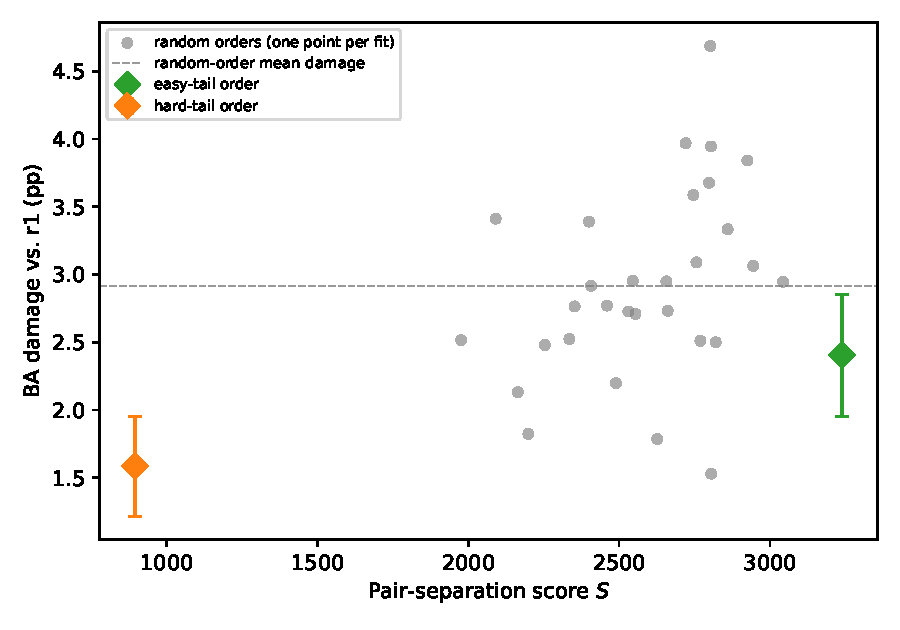
\includegraphics[width=0.78\textwidth]{gate_score_vs_damage.pdf}
\caption{The score tracks damage among random class orders but misplaces the sorted ones. Observed balanced-accuracy damage against the pair-separation score at $\rho=100$. Grey points: the 30 random class orders of the prevalence curve, one per split-draw fit, with their mean damage as the dashed line. Diamonds with 95 percent bootstrap intervals: the hard-tail order (orange) and the easy-tail order (green), each pooled over 30 fits. The easy-tail order lies to the right of every random order yet below their mean damage, which is the inversion that fails the gate.}
\label{fig:gate}
\end{figure}

\subsection{Why the sorted orders break the score}
\label{sec:why}
The inversion follows from how the sorted orders and the score are each built, and does not need a further fit to see. The easy-tail order is defined by sorting the classes on exactly the quantity the score uses as its weight: each class's balanced-arm recall $h_c$. Rank and $h_c$ are therefore perfectly monotone in that order, and perfectly monotone in the opposite direction in the hard-tail order, whereas in a random order they are unrelated.

Consider what this does to the terms of Equation~\eqref{eq:score}. In the easy-tail order the classes with the largest $h_c$ occupy the highest rank indices and thus the smallest allocations, so almost every other class sits above them and each of the resulting gaps is multiplied by a large weight. The two factors of every large term, the weight $h_c$ and the log-count advantage of the classes above $c$, are aligned across the whole order at once. In the hard-tail order the same alignment runs backwards: the large-$h_c$ classes sit at the head with almost nothing above them, their terms are close to zero, and the score collapses to 895, below every random order. A random order achieves neither alignment and lands in between.

The score consequently rewards monotone agreement between recall and rank as such. Ordering the classes by difficulty produces that agreement by construction, in either direction, and so moves the score to an extreme, while the measured damage of both sorted orders is mild, because sorting by difficulty also keeps classes of similar difficulty, and therefore many confused pairs, close together in rank \citep{queisler2026tailTcga}. What the score was meant to capture, the separation of confused pairs, and what it actually responds to most strongly, the alignment of headroom with rank, come apart precisely on the assignments that are not random.

This matters for the use the score was built for. A search over assignments does not sample the random family; it travels to the extremes of the score, far outside it. The correlation of 0.38 within random orders licenses no claim about those extremes, and the single order known to lie outside the random family is the one where the score errs most. Maximizing $S$ would therefore have produced an order chosen for a property that has not been shown to cost accuracy, and the 120 fits would have measured the damage of that order without testing the claim the study set out to test.

\section{Discussion}
\label{sec:discussion}
The candidate worst-case assignment named by the tail-assignment study \citep{queisler2026tailTcga} is not supported in this form. Written as a single directed sum over confused pairs, weighted by headroom and by log-count gap, it does not rank the three class orders whose damage is known, and the order it ranks as worst is measurably milder than average. The result is a null about the score, reached at the cost of no new fits.

The null is narrower than it may appear, and two things survive it. The pairwise reading of the damage itself is untouched: it rests on per-class recall changes measured under two fitted orders, where rectum adenocarcinoma lost 13 points of recall below colon adenocarcinoma and gained 7 points above it, and where classes whose confusion partners stayed at adjacent ranks barely moved \citep{queisler2026tailTcga}. Nothing here contradicts that. What fails is the step from that per-pair observation to a scalar summary of a whole assignment. Equally, the possibility that some assignment is markedly worse than a random one remains open; this report shows only that this particular score does not identify it.

The gate itself is the practical lesson. Its three anchor points cost nothing, because all three damages had already been fitted, and it was specified before the score was evaluated. Had the search run first, it would have consumed 120 fits and returned an order with some measured damage, and the resulting number would have been hard to interpret, since a search maximizing a proxy will return an extreme of the proxy whether or not the proxy tracks the target. Checking a proxy against known values before optimizing it is cheap in proportion to what it protects, and it is most informative when the known values include cases from outside the family the proxy was formed on.

A replacement score would need to satisfy two requirements that this one does not. It must not be maximized by monotone agreement between rank and any per-class weight, since assignments with that structure are among the mildest observed here, which suggests scoring each confused pair on its rank gap and direction in a way that does not accumulate across unrelated classes. It must also be checked against anchors that lie outside the random family, and at present only two such anchors exist, the easy-tail and hard-tail orders. Fitting one or two further deliberately constructed orders, cheap at 30 fits each, would strengthen any future gate more than another search would. Such a score would require its own pre-registration; adjusting the present one against the present gate would turn a prediction into a fit.

\section{Limitations}
\label{sec:limitations}
The gate rests on three damages, one of them an average, and is a necessary rather than a sufficient check: a score could pass it and still fail to identify the worst assignment, since ranking three known orders correctly says little about the extremes of a space of $30!$ assignments. The two sorted orders are the only available anchors outside the random family, and they are reversals of one another rather than independent constructions, so the evidence that the score misbehaves away from random orders comes from a single pair of related orders.

The damages entering the gate are not measured on a common footing. The sorted-order damages pool 30 fits each with bootstrap intervals, whereas each random-order damage is a single fit whose patient and test-set variation, at a standard deviation of 0.70 points across fits, attenuates the G3 correlation and would attenuate it even for a score that ranked assignments perfectly. G3 is reported as descriptive for that reason and carries no weight in the pass rule.

The score is evaluated on the $\rho=100$ count profile. Its ordering of assignments is invariant to the ratio up to a scale factor, so the same order maximizes it at $\rho=10$, but this invariance is a property of the score rather than a tested property of the damage, and the gate does not test whether the damage ordering itself is stable across ratios. Confusion weights and headroom come from pooled patch-level confusion counts in the balanced arm, which weight classes with many test patches more heavily and do not capture morphological similarity as a pathologist would judge it. All results are conditional on twenty patients per class, frozen Virchow2 features, multinomial logistic regression with regularization selected on validation patient-macro balanced accuracy \citep{queisler2026patientShortage}, and the three overlapping splits of TCGA-UT.
